% Working draft, 8 November 2026. Not approved for submission.
\documentclass[10pt,twocolumn,letterpaper]{article}
\usepackage[T1]{fontenc}
\usepackage[review]{cvpr}
\usepackage{amsmath,amssymb,graphicx,booktabs}
\usepackage[pagebackref,breaklinks,colorlinks,citecolor=cvprblue]{hyperref}
\definecolor{cvprblue}{rgb}{0.21,0.49,0.74}
\def\paperID{DRAFT}
\def\confName{CVPR}
\def\confYear{2027}
\newtheorem{proposition}{Proposition}
\newcommand{\E}{\mathbb{E}}
\newcommand{\Prob}{\mathbb{P}}
\title{Identity Ladder: Measuring Identity, Symmetry, and Variability in Human Images}
\author{Anonymous authors}

\begin{document}
\maketitle
\noindent\textbf{Development copy, not for submission.}
The related ISBI manuscript is under review. This draft retains shared analyses to develop the argument; their inclusion is not a determination of permissible publication overlap. An independent CVPR contribution and a compliant submission scope remain to be established.

\begin{abstract}
Human images differ across individuals, across repeated captures, and between bilateral structures of one person. A useful distance must be interpreted relative to these sources of variation, particularly when evaluating whether an inpainted region preserves individual anatomy. We develop Identity Ladder, an audit protocol combining controlled identity and nuisance comparisons, matched unrelated references, and population-mean and incorrect-detail controls. The protocol separates discrimination, residual magnitude, and target alignment without prescribing a universal biological ordering. Saved synthetic experiments expose opposite failure directions: a population-mean tissue image reaches an unrelated-reference rank of 0.995 under RMSE despite zero target residual, whereas the same simulated eye under dilation reaches 0.004. Matching the reference dilation raises the latter to 0.449 but does not establish invariance. Exploratory real-image comparisons show that representation and correspondence matter: reflecting fellow-eye fundus pixels changes their mean rank from 0.692 to 0.810, while image mean and contrast alone reach 0.919 for same-eye UPOL comparisons, close to the pixel score of 0.923. We specify how these comparisons extend to spatial variability maps and held-out inpainting evaluation. The present evidence supports an audit of similarity interpretations; the full cross-anatomy atlas, contemporary reconstruction comparison, and validation of a scalar identity measure remain unperformed.
\end{abstract}

\begin{figure*}[t]
\centering
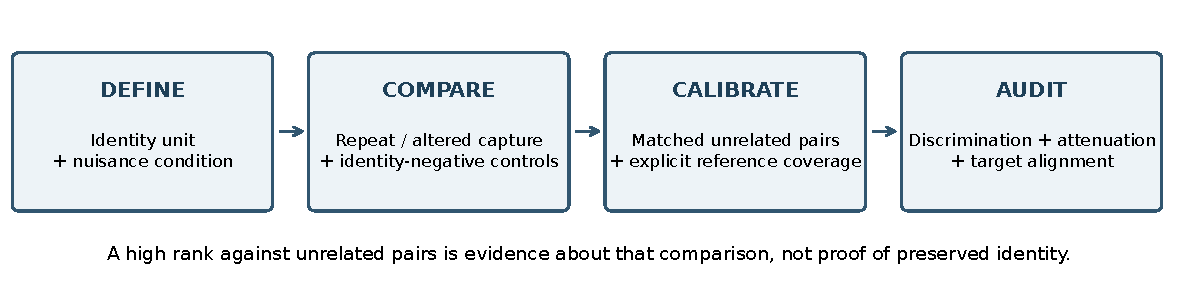
\includegraphics[width=\textwidth]{figures/audit_overview.pdf}
\caption{\textbf{Identity Ladder as an audit of interpretation.} Define what identity means for the task, construct comparisons that vary identity and acquisition separately where possible, and calibrate against unrelated references with the same measured nuisance condition. Report a profile of checks. The order of these operations is a protocol, not a learned image-generation pipeline.}
\label{fig:overview}
\end{figure*}

\section{Introduction}
Image reconstruction is often evaluated against one reference image. A small error is then used to support a stronger interpretation: that the reconstruction preserves the depicted individual. These are different claims. A population-typical image may have low error without reproducing the target's distinguishing features. Conversely, a new acquisition of the same individual may incur substantial error because of illumination, sensor, pose, physiology, or time. The relevant question is therefore not only how close two images are, but what their closeness measures.

The ambiguity matters when reconstruction is intended to preserve anatomy or biometric information. In healthy-tissue inpainting, plausible population structure and target-specific structure need not coincide. In ocular imaging, the same eye changes appearance across captures, while two eyes from the same person share both biology and acquisition conditions. A metric can respond to either source of similarity. Even a successful same-person versus unrelated-person comparison may exploit capture shortcuts if the comparison groups do not share acquisition conditions.

Bilateral anatomy makes the question particularly concrete. A left hemisphere and a right hemisphere belong to one person but are not identical copies; two irises belong to one person but are distinct biometric instances. A face reflected about its midline supplies a within-image asymmetry measurement, whereas an independently captured face also includes acquisition variation. These comparisons should therefore be described by the structures and conditions they change. Calling all of them \emph{same identity} conceals the distinction the metric is supposed to resolve.

We formulate this problem as a metric audit. Identity Ladder organizes repeated captures, nuisance interventions, later observations, bilateral or family relationships where available, and unrelated comparisons. Population means and wrong-detail controls test complementary failure modes. Matched unrelated references express each distance as an interpretable rank, but the audit explicitly distinguishes this calibration from invariance or validation of identity preservation.

Our methodological contribution is the organization of these checks into a single evaluation protocol. The empirical contribution at this stage is a set of synthetic counterexamples and acquisition-aware comparisons of saved fundus and iris representations. Together they separate three questions that a single similarity score conflates: does a representation discriminate controlled identity relationships, does an output retain individual variation, and is the retained variation aligned with the target? The percentile transformation and its AUC interpretation are established statistical tools, as is the squared-error preference for a conditional mean. Neither is claimed as a new distance.

The evidence comprises saved synthetic tissue and eye experiments and exploratory ocular-image pilots. It supports a failure analysis and a protocol, rather than a universal ordering of biological similarity. In particular, we do not infer a validated identity score from a hand-designed simulator. The absence of held-out comparisons on outputs of modern reconstruction methods remains a material limitation of the present draft.

The intended next contribution is a common benchmark across brain, external-eye, fundus, face, and pupil-related views. Its central visual artifact is an atlas separating repeat, bilateral, and between-person spatial differences. Section~\ref{sec:extension} specifies that extension so that its design is reviewable before further scoring; those proposed experiments are not included among the measured results.

\section{Related work}
\paragraph{Distortion and perception.}
The perception--distortion tradeoff formalizes the distinction between average reference distortion and distributional perceptual quality~\cite{blau2018}. SSIM~\cite{wang2004} and learned perceptual distances such as LPIPS~\cite{zhang2018lpips} address aspects of image similarity. Identity preservation is an additional task-specific interpretation: an image may be plausible yet depict the wrong individual. Our audit does not assume that either pixel or learned features resolve that interpretation without controls. It also does not claim that perceptual metrics fail on the present experiments, because those comparisons have not yet been run.

\paragraph{Recognition and metric selection.}
Classical iris recognition compares normalized iris texture to distinguish eyes~\cite{daugman2004}. This highlights the need to specify whether the identity unit is an eye or a person. A fellow eye is a different biometric instance even when it belongs to the same person. More broadly, metric suitability depends on the intended task and data properties, as emphasized by Metrics Reloaded~\cite{maierhein2024}. We extend this task-first reasoning to a profile of identity, nuisance and collapse checks, rather than proposing a replacement for all recognition or reconstruction metrics.

\paragraph{Conditional calibration.}
Reference-distribution placement values and covariate-adjusted ROC analysis are established ways to interpret markers relative to controls~\cite{pepe2005,janes2009}. Our unrelated-reference score is an application of that machinery to image pairs. Its value depends on the control population, matching variables and weighting. The novelty sought here is the audit design around the calibrated score, not the score's statistical definition. GRAPE~\cite{huang2023grape} and UTIRIS~\cite{hosseini2010} provide exploratory ocular comparisons, and the fundus pilot uses released RETFound features~\cite{zhou2023retfound}.

\section{Identity Ladder audit}
\subsection{Identity units and comparison conditions}
Let $x_{u,s}$ be an image of identity unit $u$ under measured acquisition condition $s$. A unit may be a person, an eye, or a specified anatomical structure. The definition must be fixed before scoring. Let $d(x,y)$ be a distance in a fixed representation, with smaller values denoting greater similarity. Similarity measures are oriented consistently before calibration.

The audit records comparisons that isolate different sources of variation: a repeated capture under closely matched conditions; the same unit with an altered acquisition condition; the same unit at a later time; a related unit, such as the fellow eye or a family member; and unrelated units. A population mean and a candidate with incorrect individual detail are additional negative controls. A mean is not a biological rung and need not lie at the bottom of a distance ranking.

The term ladder describes a collection of interpretable comparisons, not a guaranteed total order. A repeat and a matched unrelated comparison support a discrimination question. A cross-device comparison supports a nuisance-sensitivity question. Whether a fellow eye should be closer than a later capture of the same eye depends on the representation and identity unit; it is not prescribed. Family relationships require verified metadata, and unknown zygosity cannot be turned into monozygotic or dizygotic labels. An unavailable rung is reported as unavailable.

\subsection{Matched unrelated-reference calibration}
For target $x$ and candidate $y$, let $q$ describe the measured condition of the pair, such as its unordered camera pair and eye relationship. Let $D_q$ be a distance from an unrelated-reference comparison satisfying that condition. Define
\begin{equation}
c_q(x,y)=\Prob\{D_q>d(x,y)\}
 +\tfrac12\Prob\{D_q=d(x,y)\}.
\label{eq:calibration}
\end{equation}
With a finite reference panel, probabilities are empirical proportions. A value near one means the candidate is closer than almost all members of that panel. It is not a probability that identity was preserved. Under exchangeability, an independently drawn unrelated comparison has expected score $1/2$, including ties. An anchor assigned $1/2$ by construction is not an independent validation of the calibration.

The mean score over candidate comparisons has a pairwise discrimination interpretation. If each candidate uses the same reference distribution, it is the usual AUC. With target-dependent or condition-dependent references, it is a weighted average of conditional discrimination probabilities. It need not equal an AUC computed by pooling all candidates and strangers. We therefore report the reference construction and weighting alongside the score.

Calibration cannot repair an unsuitable representation. Within a fixed reference stratum, Eq.~\ref{eq:calibration} is monotone in distance, with possible ties from finite resolution. It cannot reverse an ordering produced by $d$. A strictly increasing transform of distance produces the same score. A change in the reference condition can change the score, but does not remove nuisance information from the representation.

Exact observed matching is preferable to a binary ``same versus different sensor'' indicator when several devices or spectra are present. When a matching stratum has no unrelated references, the audit abstains for that stratum and reports coverage. Pooling unmatched pairs changes the estimand. Matching also cannot remove unmeasured session effects, disease progression, or acquisition factors shared only by the positive pair.

\subsection{Population collapse and target alignment}
Let $x=\mu+\delta$ in a Euclidean representation, where $\mu$ is a population expectation and $\E\delta=0$. Let $V=\E\|\delta\|^2/D$ in $D$ dimensions. These assumptions yield a simple diagnostic counterexample.

\begin{proposition}[Population-mean advantage]
For an equal-variance donor $y=\mu+\delta'$ with $\E\langle\delta,\delta'\rangle/D=rV$, the expected per-dimension squared error is $2V(1-r)$, while the error of $\mu$ is $V$. Thus the population mean has smaller expected squared error whenever $r<1/2$.
\end{proposition}
\noindent The result follows by expanding $\|\delta-\delta'\|^2$. For an independent donor $r=0$, the ratio is $1/2$. A finite independent sample mean has estimation variance and need not attain this exact value. Likewise, unequal donor variances alter the expression. The result concerns expected error, not the ranking of every target or an arbitrary calibrated AUC.

For a predictor conditioned on visible context $z$, squared error is minimized by $\E[x\mid z]$. A population mean is therefore a useful collapse control, but need not be the best context-conditioned baseline. Beating an unconditional mean alone does not establish recovery of the hidden individual detail.

To describe attenuation and incorrect detail separately, use an independently estimated mean $\hat\mu$, let $a=x-\hat\mu$ and $b=y-\hat\mu$, and report
\begin{equation}
A=\frac{\|b\|}{\|a\|},\qquad
P=\frac{\langle b,a\rangle}{\|a\|^2},\qquad
O=\frac{\|b-Pa\|}{\|a\|}.
\label{eq:residuals}
\end{equation}
Here $A$ measures residual magnitude, $P$ target-directed projection, and $O$ the orthogonal component. They are descriptive coordinates, not a validated scalar identity score. A noisy candidate can have $A\simeq1$ while $P\simeq0$. Residual cosine alone misses amplitude loss: on the oracle shrinkage path $y_\lambda=\hat\mu+\lambda(x-\hat\mu)$ it remains one for every $\lambda>0$, while $A=P=\lambda$.

This path deliberately uses the known target. Its algebra is an implementation check, not evidence of external validity. If $\|a\|$ is small relative to repeat-measurement variability, the ratios are unstable and should be flagged as unresolved. A repeat-derived resolution threshold remains to be established. The decomposition also requires a fixed Euclidean representation; it cannot be transferred to arbitrary distances without a corresponding definition.

\subsection{Reporting and uncertainty}
The audit reports raw distances, calibrated ranks, residual diagnostics where defined, and all unavailable conditions. Targets, template contributors and reference donors must be separated at the relevant identity or family level. Nuisance-only features, such as image mean and standard deviation, test whether a high score requires individual structure at all.

Repeated pairs do not create independent participants. Confirmatory intervals should resample participants or families, preserve within-cluster relationships and reconstruct the calibration reference within each resample. Pair-weighted and participant-weighted summaries answer different questions and should not be silently substituted. The exploratory pilot intervals below are inherited from saved patient/person-bootstrap outputs; their treatment of reference-pool uncertainty has not been certified for a final benchmark.

\subsection{Bilateral correspondence and distance representation}
\label{sec:bilateral}
Let $L_{p,t}$ and $R_{p,t}$ denote observed left and right structures of person $p$ at acquisition $t$, and let $H$ be a fixed reflection/correspondence operator. The within-acquisition quantity $d(L_{p,t},HR_{p,t})$ measures observed bilateral difference under shared capture conditions. Comparing $L_{p,t}$ with $HR_{p,t'}$ at another acquisition changes both side and capture. Neither quantity alone identifies a biological symmetry component. A useful control repeats the same correspondence operation on unrelated opposite-side pairs; otherwise a change in score can arise from transforming only the candidate.

The interpretation also depends on representation. Euclidean pixel distances retain local photometry and correspondence errors. A normalized iris code targets texture in a specific coordinate system. A learned fundus representation may suppress some left--right layout differences while retaining acquisition information. These are hypotheses for controlled comparison, not guarantees supplied by the representation name. We therefore retain unreflected and reflected pixel conditions separately and avoid selecting the better condition after observing identity scores.

Monotone-equivalent distances should not be counted as independent successful baselines. In particular, unit-normalized features satisfy $\|u-v\|^2=2(1-u^\top v)$, so cosine distance and squared Euclidean distance produce the same ordering on those features. Likewise, MSE and RMSE have identical within-case ordering. PSNR has that equivalence only when its range and preprocessing are fixed; image-dependent range selection and clamping must be examined separately. Raw values remain useful for diagnosing residual attenuation even when their calibrated ranks coincide.

\section{Experiments}
\subsection{Saved synthetic experiments}
\paragraph{Controlled shrinkage.}
The population-null experiment contains three seeds and eight independent targets per seed per modality: 24 tissue families and 24 eye identities. Each seed uses separate template and reference pools of 40 and 24 families or people. Five shrinkage values, $\lambda\in\{1,.75,.5,.25,0\}$, share the same target and are not five independent identities. The tissue prior scale is 0.25. A wrong-detail control starts with a residual orthogonal to the target and matched in norm before nonnegativity clipping; diagnostics describe the actual clipped image.

The saved experiment computes the nine intensity outputs of the BraTS inpainting package, version 0.0.12, with torchmetrics 1.9.0. These are two-dimensional diagnostic adaptations, not official three-dimensional challenge submissions. We focus on RMSE and SSIM here; multiple monotone variants of squared error do not constitute independent evidence. The experiment does not evaluate a trained reconstruction model.

\begin{table}[t]
\centering
\caption{\textbf{Attenuation versus wrong detail.} Means over 24 independent synthetic targets per modality. $c$ is the unrelated-reference rank; $A$ and $P$ are Eq.~\ref{eq:residuals}. A high $c$ need not imply a retained target residual.}
\label{tab:null}
\footnotesize
\setlength{\tabcolsep}{3pt}
\begin{tabular}{@{}llrrrr@{}}
\toprule
 & Candidate & RMSE $c$ & SSIM $c$ & $A$ & $P$ \\
\midrule
Tissue & Repeat capture & 1.000 & 1.000 & 0.999 & 0.974 \\
Tissue & 50\% residual & 1.000 & 1.000 & 0.500 & 0.500 \\
Tissue & Population mean & 0.995 & 0.950 & 0.000 & 0.000 \\
Tissue & Wrong detail & 0.566 & 0.184 & 1.000 & -0.000 \\
\midrule
Eyes & Repeat capture & 1.000 & 1.000 & 1.000 & 0.988 \\
Eyes & 50\% residual & 0.998 & 1.000 & 0.500 & 0.500 \\
Eyes & Population mean & 0.797 & 0.835 & 0.000 & 0.000 \\
Eyes & Wrong detail & 0.389 & 0.085 & 0.972 & 0.000 \\
\bottomrule

\end{tabular}
\end{table}

\paragraph{Pupil intervention.}
A separate eye simulator keeps latent identity parameters fixed while increasing pupil radius by 30\% and deforming iris texture in normalized radial coordinates. Three seeds contain 32 target people each, for 96 independent synthetic targets, with separate template and reference pools. Images are $96\times96$, evaluated in a central $64\times64$ mask against 16 unrelated donors per target. The comparison is also recalibrated using dilated unrelated references. Pupil masks are obtained by smoothing and thresholding. This controlled model is not a study of human physiology or a validated biometric.

\paragraph{Label sensitivity.}
The label-space experiment varies a population prior over $0,0.25,1$ and uses two illustrative latent variance settings. Five seeds contain 60 two-person families each. Shared draws across settings support paired comparisons; they do not multiply the number of independent families. A smoothed threshold segmenter produces two-class labels, compared with labels of the true image using Dice and simple geometry/topology descriptors. Seed ranges are descriptive minima and maxima, not confidence intervals.

\begin{figure*}[t]
\centering
\includegraphics[width=.92\textwidth]{figures/visual_tissue_rebuilt.pdf}
\caption{\textbf{Synthetic tissue controls.} Saved, fixed-index example showing target context, enlarged candidate regions and threshold segmentations. The population mean suppresses individual detail. Example-level scores need not equal the cohort means in Table~\ref{tab:null}. This is synthetic random-field tissue, not an MRI scan or a trained inpainting output.}
\label{fig:tissue}
\end{figure*}

\subsection{Exploratory ocular pilots}
The fundus pilot uses 631 GRAPE images and released RETFound features. Comparisons distinguish the same eye across visits from fellow eyes in one visit. Unrelated references are matched on the exact unordered camera pair and eye relationship. Visits are defined from acquisition date. Table~\ref{tab:ocular} reports the saved pair-weighted summaries and patient-bootstrap intervals with the number of contributing patients for each condition; these subsets differ.

The UTIRIS pilot uses near-infrared iris images and a classical normalized phase-code representation: a $16\times128$ rubber-sheet strip, one-dimensional log-Gabor filtering, two-bit phase and minimum Hamming distance over $\pm6$ shifts. After exclusion of recorded eye-label conflicts, 778 images enter the saved near-infrared analysis, and segmentation passes its QC rule for approximately 94\%. Same-eye and fellow-eye pairs are calibrated against unrelated people under the same sensor and eye condition. We use the plain fellow-eye comparison, rather than selecting the flipped version for a higher score. Visible-spectrum results are secondary because segmentation acceptance is much lower.

The saved pixel pilot provides additional representation controls on UPOL and UTIRIS. Images are reduced to $16\times16$ grayscale arrays. The photometric control uses only the image mean and standard deviation; a separate condition standardizes each image's pixels to zero mean and unit standard deviation. UPOL contains 384 images from 64 people. The within-NIR UTIRIS pixel comparisons involve 78 people. These pair sets differ from the phase-code QC subset, so the phase-code and pixel scores are not treated as a paired ranking of methods.

For GRAPE, the reflected-pixel condition reflects the actual fellow-eye image and applies the same transformation to unrelated opposite-eye references. Same-eye distances remain unchanged. RETFound uses the released features; reflected-image RETFound features were not recomputed. The saved representation comparisons use the same recorded pair counts within a dataset and condition. All summaries remain pair-weighted, and a common count does not make repeated pairs independent.

No real-MRI ordering result is used as primary evidence here. The previous MRI audit identified protocol confounding and unresolved middle comparisons. Human-image exemplars are not reproduced; the present draft uses aggregate ocular outputs and synthetic illustrations only.

\section{Results}
\subsection{A high rank can survive residual collapse}
On synthetic tissue, the population mean reaches RMSE $c=0.995$ and SSIM $c=0.950$, despite zero residual amplitude and projection (Table~\ref{tab:null}). Retaining only half the target residual yields $c=1.000$ under both metrics. This is saturation relative to the selected unrelated panel. It does not mean that the half-residual image equals the target: its raw RMSE is nonzero. The exact target has zero error, so describing the two as indistinguishable from truth would overstate the result.

The eye simulator shows the same direction with a smaller mean advantage: the population mean scores 0.797 under RMSE and 0.835 under SSIM. Thus the magnitude of collapse tolerance depends on the image generator and reference distribution. The wrong-detail tissue control has residual amplitude 1.000 but projection approximately zero; its scores fall to 0.566 and 0.184. Magnitude alone therefore cannot establish that a candidate preserves the correct individual detail.

\subsection{Matching does not establish invariance}
In the pupil experiment, repeat capture reaches $c=1.000$ under RMSE and SSIM. The same eye after dilation reaches 0.004 and 0.006 against normal-pupil unrelated references. Dilation-matched references raise these scores to 0.449 and 0.432 (Fig.~\ref{fig:pupil_scores}), far below the simulated repeat level. The latent identity parameters are unchanged by construction, yet the representation responds strongly to the intervention.

The independent population mean scores 0.794 under RMSE and 0.842 under SSIM in this experiment. These numbers come from a different design than the shrinkage experiment in Table~\ref{tab:null} and should not be combined into one estimate. Pupil component-count error is zero for every candidate and therefore yields $c=0.5$, even for repeats. A topology descriptor can be uninformative rather than protective against identity collapse.

\begin{figure}[t]
\centering
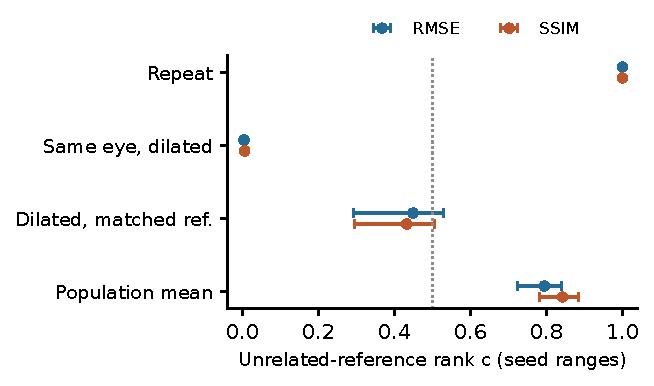
\includegraphics[width=\columnwidth]{figures/pupil_scores.pdf}
\caption{\textbf{Two failure directions in one simulator.} An identity-preserving dilation is penalized, while the population mean retains a high score. Bars are minima/maxima of three seed means, not confidence intervals. The vertical line is the unrelated anchor. Matching the reference intervention changes calibration without repairing the representation.}
\label{fig:pupil_scores}
\end{figure}

\begin{figure*}[t]
\centering
\includegraphics[width=\textwidth]{figures/pupil_fixed_example.pdf}
\caption{\textbf{Fixed synthetic eye example.} Seed 201, target index zero, chosen independently of its metric results. Rows show intensity, estimated pupil mask and contour agreement. These are example-level values; cohort results are in Fig.~\ref{fig:pupil_scores}. Pupil shape alone does not define eye identity, and fellow-eye similarity reflects the simulator's chosen shared parameters.}
\label{fig:pupil}
\end{figure*}

\subsection{Label agreement has a conditional failure mode}
Across the label sensitivity conditions, mean-image RMSE ranks remain approximately 0.995--0.997. The paired Dice comparison with a simulated monozygotic co-twin depends on the prior and latent variance setting. In the low-genetic-share setting with prior scale one, the mean-minus-co-twin difference is $+0.215$, with five-seed range $[+0.150,+0.284]$. At prior scale 0.25 the range crosses zero; without a prior there is no stable direction. The higher-genetic-share setting favors the co-twin on Dice in every tested prior condition.

This supports a conditional empirical observation in the simulator. Pointwise label accuracy is maximized by a conditional modal label, but Dice is a ratio with a spatially coupled denominator; the accuracy argument does not establish a general Dice theorem. Component counts of the mean are approximately unrelated-like, with $c$ around 0.50--0.56, but rare holes, ties and mask-border cuts limit interpretation. No trained-segmenter or topology-based identity validation follows from these results.

\begin{figure*}[t]
\centering
\includegraphics[width=.92\textwidth]{figures/label_fixed_example_folding.pdf}
\caption{\textbf{Synthetic label-space comparison.} A fixed folding-like example includes other-day and opposite-side donors as well as mean and unrelated controls. Labels come from a threshold segmenter. The experiment tests possible behavior of overlap and simple shape descriptors; it does not establish their behavior on real brain segmentations.}
\label{fig:labels}
\end{figure*}

\begin{table*}[t]
\centering
\caption{\textbf{Exploratory ocular pilots.} Saved pair-weighted means with original 95\% patient/person-bootstrap intervals. $N$ is contributing patients or people, not images; pair counts are dependent. The reference populations and representations differ between datasets, so equal values are not a common biological scale. These intervals do not certify full uncertainty from estimating the reference pool.}
\label{tab:ocular}
\small
\begin{tabular}{@{}llrrl@{}}
\toprule
Dataset & Comparison & $N$ & Pairs & Mean $c$ [95\% interval] \\
\midrule
GRAPE & Same eye, later visit, same camera & 71 & 250 & 0.873 [0.832, 0.906] \\
GRAPE & Same eye, later visit, other camera & 83 & 398 & 0.777 [0.735, 0.812] \\
GRAPE & Fellow eye, same visit, same camera & 119 & 276 & 0.907 [0.883, 0.930] \\
\midrule
UTIRIS & Same eye, same sensor & 76 & 1453 & 0.913 [0.889, 0.938] \\
UTIRIS & Fellow eye, same sensor & 75 & 1789 & 0.668 [0.622, 0.710] \\
\bottomrule

\end{tabular}
\end{table*}

\subsection{Real-image pilots require acquisition-aware interpretation}
In GRAPE, same-eye later-visit comparisons score 0.873 with the same camera and 0.777 across cameras. These are descriptive summaries over different patient subsets, not a causal camera-effect estimate. Camera, acquisition era and time gap are coupled, and disease progression was not controlled. The same-visit fellow eye scores 0.907, illustrating why a naive biological ordering cannot be imposed. Shared visit conditions and distinct subsets complicate comparison with same-eye longitudinal observations.

In UTIRIS near-infrared images, the phase code scores 0.913 for the same eye and 0.668 for the fellow eye under the recorded matching scheme. This separates eye-level and person-level relationships descriptively. The fellow-eye signal does not by itself prove shared identity-specific iris texture: estimated geometry, segmentation and residual capture effects remain possible contributors. Earlier pixel-level pilots also found that nuisance-only intensity summaries reproduced much of the apparent similarity. Strong performance on the calibration scale therefore requires examination of which features produce it.

\begin{table*}[t]
\centering
\caption{\textbf{Representation changes the interpretation of a high score.} Saved mean calibrated ranks for same-unit ($s$) and fellow-eye ($b$) comparisons. $N_s/N_b$ counts contributing people and $P_s/P_b$ dependent pairs. GRAPE uses the same eye at a later visit and the fellow eye in the same visit, both with the same camera; iris datasets use the same sensor. Rows within a dataset use the same recorded pair counts. No paired significance test between representations is asserted.}
\label{tab:representations}
\small
\begin{tabular}{@{}llccrr@{}}
\toprule
Dataset & Representation & $N_s/N_b$ & $P_s/P_b$ & Same-unit $c$ & Fellow-eye $c$ \\
\midrule
GRAPE & Pixels & 71/119 & 250/276 & 0.714 & 0.692 \\
GRAPE & Pixels, fellow eye reflected & 71/119 & 250/276 & 0.714 & 0.810 \\
GRAPE & RETFound & 71/119 & 250/276 & 0.873 & 0.907 \\
\midrule
UPOL & Image mean and SD & 64/64 & 384/576 & 0.919 & 0.884 \\
UPOL & Pixels & 64/64 & 384/576 & 0.923 & 0.805 \\
UPOL & Standardized pixels & 64/64 & 384/576 & 0.875 & 0.719 \\
\midrule
UTIRIS NIR & Image mean and SD & 78/78 & 1587/1967 & 0.793 & 0.764 \\
UTIRIS NIR & Pixels & 78/78 & 1587/1967 & 0.846 & 0.713 \\
UTIRIS NIR & Standardized pixels & 78/78 & 1587/1967 & 0.785 & 0.616 \\
\bottomrule

\end{tabular}
\end{table*}

\subsection{Photometric controls and reflection reveal different signals}
Table~\ref{tab:representations} compares representations within recorded comparison conditions. In UPOL, image mean and standard deviation yield same-eye $c=0.919$ and fellow-eye $c=0.884$. The corresponding pixel scores are 0.923 and 0.805. Standardizing image intensity changes them to 0.875 and 0.719. Thus a high same-eye rank can also be obtained without a spatial texture representation, and the relative apparent strength of fellow-eye similarity changes with preprocessing. The control demonstrates a photometric signal associated with the comparison labels; it does not establish that the signal is entirely acquisition nuisance or quantify the fraction of texture information.

UTIRIS NIR shows a related but distinct profile. The photometric control scores 0.793 for the same eye and 0.764 for the fellow eye; pixels score 0.846 and 0.713. With per-image standardization, the scores become 0.785 and 0.616. Standardization therefore does not uniformly improve the measured discrimination. It changes the information used by the distance and may remove both acquisition variation and person-associated appearance. These summaries do not identify a preferred normalization without a prespecified target task.

In GRAPE, same-eye later-visit pixels score 0.714, whereas fellow-eye same-visit pixels score 0.692. Reflecting the fellow-eye pixels changes the latter to 0.810 while leaving the same-eye score unchanged. RETFound produces 0.873 and 0.907 for the two conditions. Reflection changes correspondence and its matched reference together; the observed rank change is not a direct estimate of anatomical symmetry or an effect size attributable only to the candidate image. The differing profiles motivate comparison-specific interpretation: representations can emphasize different aspects of shared appearance, and the same-unit and fellow-eye conditions also differ in acquisition timing.

\section{Cross-anatomy benchmark extension}
\label{sec:extension}
The following specification defines proposed experiments rather than additional findings. The intended domains are brain MRI, external-eye or iris images, fundus photographs, faces, and pupil geometry. These are anatomical views, not necessarily independent cohorts: pupil contours and iris texture can come from the same eye images. Face comparisons and measured human pupil responses are not present in the saved result set. Unsupported conditions should remain unavailable rather than be filled by synthetic examples labeled as real evidence.

\subsection{Spatial difference atlas}
The proposed main figure places anatomical views in rows and repeat-capture, bilateral, and unrelated-person differences in columns. An individual-residual panel compares held-out images with an independently estimated population template. For a valid spatial location $v$, define a squared residual after prespecified within-domain correspondence $T$,
\begin{equation}
e_{ab}(v)=\frac{1}{C}\sum_{c=1}^{C}
\big[(T_a x_a)(v,c)-(T_b x_b)(v,c)\big]^2.
\label{eq:spatial}
\end{equation}
Here $C$ is the number of channels. For condition $q$, let $\mathcal{P}_{p,q}(v)$ contain the eligible pairs of participant $p$ that are valid at $v$. First average $e_{ab}(v)$ within each participant, then average these summaries with equal participant weight and take the square root. Report the number of valid contributors at each location. Use family-level weighting if families, rather than people, define the independent sampling units.

These maps summarize observed differences under a specified preprocessing procedure. Subtracting a repeat map from an unrelated map does not automatically isolate identity variance. Acquisition, progression, registration error and unequal variances can contribute to the contrast. Registration should therefore be fixed independently of the tested metric, with sensitivity analysis for correspondence strength. A nonlinear registration that removes local anatomical variation may reduce exactly the differences the benchmark intends to measure.

Each anatomical row should share a color scale across its comparison columns, while retaining a domain-specific unit and scale. Quantitatively different modalities should not share an unlabeled absolute scale. Invalid background and interpolation padding are excluded. Examples, crops and display windows are fixed independently of their score rankings. A compact adjacent metric profile connects the spatial observations to discrimination results; a scalar feature distance is not rendered as a spatial error map without an explicit attribution definition.

\subsection{Inpainting as the application test}
The application experiment should use held-out regions whose original images are observed. Candidates include interpolation, an independently estimated template fill, actual contralateral anatomy where meaningful, a matched unrelated donor, and trained reconstruction outputs. Template, reference, training and test roles must be separated at the identity level, with family separation where relevant. Known-target shrinkage remains a diagnostic control, not a competing reconstruction method.

Evaluation should distinguish the masked interior from a boundary band and vary prespecified mask locations and sizes. For each candidate, report reference distortion, calibrated discrimination, residual amplitude and target alignment where defined, and structure-specific measurements. A method can preserve a boundary while replacing the interior with typical tissue, or retain realistic but incorrect detail. Multiple stochastic outputs from one case remain clustered within that case. The comparison should ask whether metric rankings agree with held-out identity evidence, without treating closeness to a single reference as a complete oracle for all plausible hidden anatomy.

\section{Discussion}
The audit exposes two routes to a misleading identity interpretation. A representation can favor a population-typical image after target detail has disappeared, or it can penalize a nuisance intervention while identity is held fixed. Calibration alone does not resolve either route. Residual amplitude detects attenuation but confuses target detail with wrong detail; projection adds target alignment but depends on the chosen representation and a usable residual noise floor. Simple topology may detect a change in one setting and tie on every candidate in another.

These observations favor a profile of task-specific checks over an unsupported scalar identity score. Repeat comparisons establish a measured resolution condition. Nuisance-only controls test shortcuts. Matched unrelated comparisons provide a reference for discrimination. Mean and wrong-detail controls distinguish loss of variation from incorrect variation. Biological relationships supply additional questions when metadata and sample size support them; they do not define a universal calibration target.

The real-image controls sharpen the distinction between recognizing a comparison condition and recovering individual anatomy. A global photometric descriptor can discriminate repeated captures when person and capture conditions remain associated. Conversely, removing global photometry can lower an identity-associated score as well as nuisance sensitivity. Similarly, reflection can improve correspondence without establishing that the two structures share the same biometric identity. These findings argue for documenting what changes between each pair of images, rather than treating a larger calibrated rank as sufficient evidence of a better identity measure.

For inpainting, the practical consequence is that a reconstruction leaderboard should state which aspect of similarity its distances assess. Strong reference fidelity, realistic population detail and correct individual detail are separate endpoints. Their disagreement is an informative result that a benchmark should expose, rather than resolve by choosing an unvalidated weighted sum. The planned atlas provides spatial context for this question; its value will depend on measured repeat variability, adequate matching and transparent missing-condition coverage.

\paragraph{Evidence limits.}
The synthetic fields, noise and variance components are hand-designed and not calibrated to human anatomy. Oracle shrinkage makes the expected residual coordinates true by construction. Threshold segmentations do not substitute for real downstream models. The ocular pilots are exploratory, depend on estimated preprocessing and inherited intervals, and do not evaluate generated outputs. The present evidence therefore demonstrates possible failure modes and motivates an audit; it does not show that the proposed diagnostics reliably rank reconstruction methods on a held-out population.

A stronger benchmark requires prespecified endpoints, held-out identity and reference pools, repeat-derived thresholds, nuisance-normalized representations, and comparisons with contemporary perceptual and foundation-model distances. It must also score outputs of actual reconstruction methods and document condition-specific coverage. If broad applicability to natural-image reconstruction is claimed, that claim needs evidence in an appropriate nonmedical task. No such additional results are asserted here.

\paragraph{Ethics and data.}
The real-image analyses use existing aggregate outputs from ocular research datasets. No participant images, identifiers or newly reconstructed human anatomy are included in this draft. Re-identification-related measurements can expose sensitive information even when analysis uses accessible data. Dataset permissions, the basis for secondary analysis and institutional review requirements must be confirmed before submission; an ethics approval or exemption is not asserted here. Template and reference construction should also exclude related people from target pools where family information is relevant.

\section{Conclusion}
Identity Ladder asks what evidence supports interpreting image similarity as preservation of an individual. Synthetic controls distinguish attenuation from incorrect detail, while saved fundus and iris comparisons show how photometry, representation and correspondence change the meaning of a high score. The protocol separates these questions and specifies a spatial atlas and inpainting extension. Completing that empirical benchmark, validating a combined identity measure and evaluating modern reconstruction outputs remain open work.

\clearpage
\section*{LLM Usage Statement}
OpenAI Codex assisted with restructuring this working manuscript, drafting and revising prose, inspecting saved aggregate results, and writing manuscript-preparation code. The source project records earlier Claude assistance with code, literature checking and draft text. AI assistance was not used to create new experimental observations in this writing session. This disclosure describes the working draft; the authors must verify the text, citations, numerical provenance and final scope before submission.

{\small
\bibliographystyle{ieeenat_fullname}
\bibliography{refs}
}

\end{document}
